\section{Block boolean flags strategy in Generate phase}

% Explains the generation phase 
% We can omit the explanation part, we can start in 'We observed...'
The EMS-GT algorithm follows the pattern-driven approach where it exhaustively tests the $4^l$ bit-array of possible motifs. It quickly filters the $4^l$ bit-array in the Generate phase by intersecting the $d$-neighborhood of the first $n'$ sequences. EMS-GT maintains two $4^l$ bit-array during the Generate phase. The first array holds the remaining candidate motifs and the second array holds the $d$-neighborhood of the current sequence. For every sequence in the first $n'$ sequences, we generate its $d$-neighborhood by blocks of bits settings. Then we intersect the $d$-neighborhood with the candidate motifs array, the resulting set will be the new candidate motifs array. We observed that at some point in the Generation phase, candidate motifs array has numerous empty blocks of $l$-mers. Applying block bits setting in this part of the neighborhood array will be useless since we already know that there is no candidate motifs in that block. An efficient way is to focus the neighborhood generation on those blocks where there are still candidate motifs. We have implemented a block boolean flags strategy that tracks these empty blocks in the candidate motifs array.

\subsection{Maintaining block boolean flags for the candidate motifs array}
We divide the candidate motifs array into groups of $4^k$ $l$-mers. The $k$ value should be the same with the one used in the block neighborhood generation strategy. In this study we used $k = 5$. For each group of $4^k$ $l$-mers, we assigned a boolean flag that tells if the group is empty or not. Everytime we update the contents of the candidate motif array, we also update the boolean flags for empty blocks in that array. Figure \ref{fig:boolean-flags} illustrates the way of grouping these $4^k$ $l$-mers and its corresponding block boolean flags.

% if else settings in block flag -- 1 if there is still candidate motifs 0 if empty.

\begin{figure}[h]
	\centering
	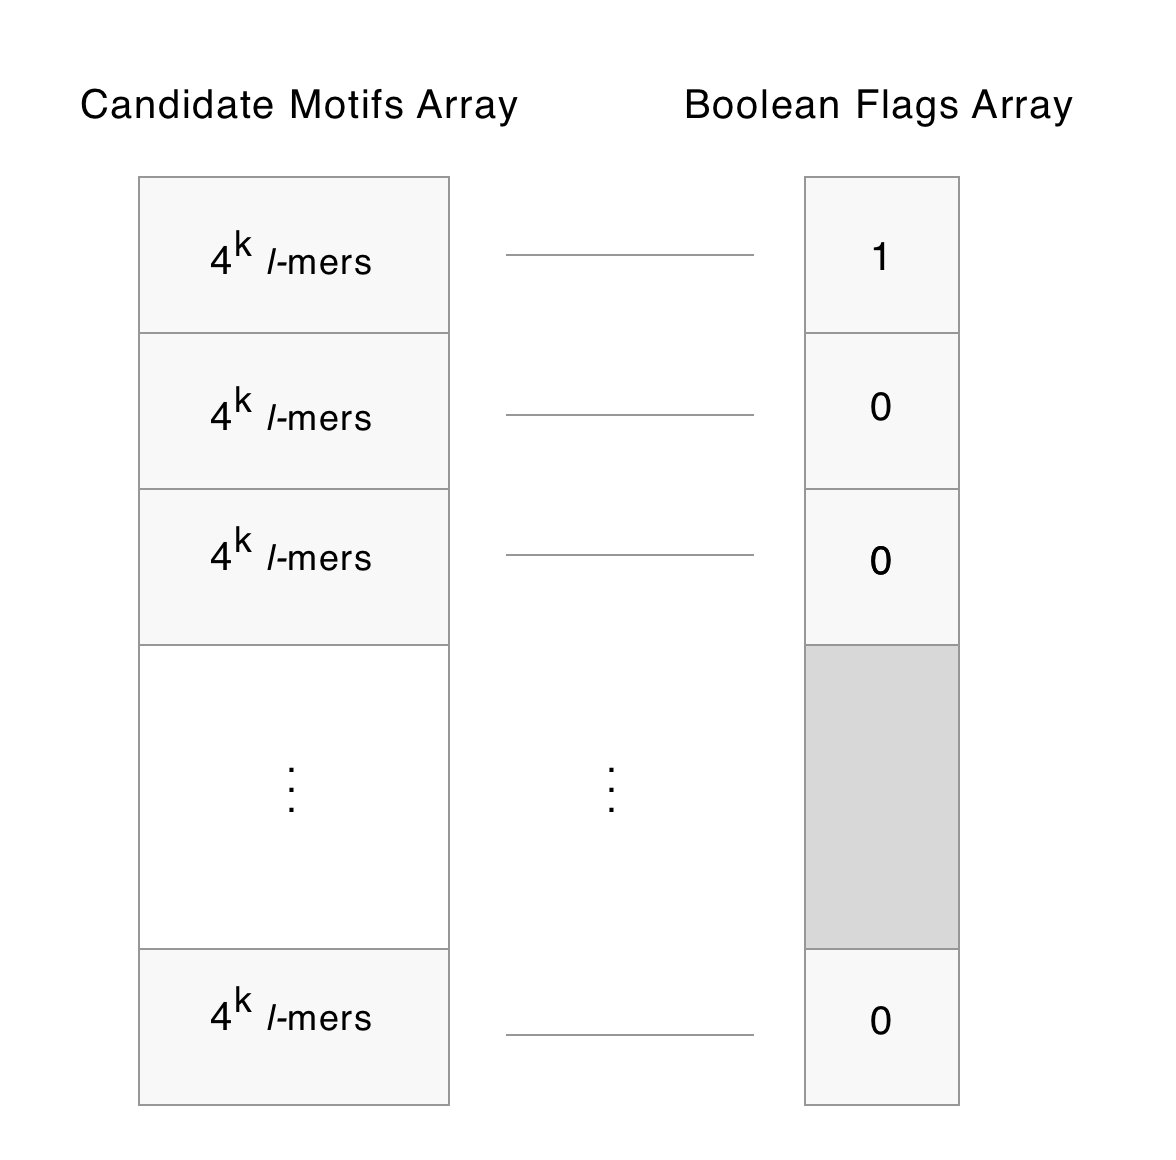
\includegraphics[width=3.5in]{contents/00_images/boolean-flags}\vspace*{5pt}
	
	\caption{Assigning boolean flags for every $4^k$ $l$-mers block in the candidate motifs array.}
	\label{fig:boolean-flags}
\end{figure}

\subsection{Usage of block boolean flags strategy}

% Rephrase 
The improved $d$-neighborhood generation uses a pre-generated block patterns of size $4^k$ $l$-mers. Given these patterns, we recursively generate all possible prefix of the given $l$-mer of length $l - k$. These prefix values represents the row start value where the block bits setting will be applied. For each prefix value, we check if can skip the block bits setting by checking if the block is empty using its assigned block boolean flag. If the prefix value is not equal to the row start value of the block the boolean flag is representing, then we need to consider also the next boolean flag since the block bits setting will overlap, unless it is the last block in the array. Figure 4.\ref{fig:block-flag-settings} shows the two scenarios we consider in skipping block bits setting.

%  --

% Make this the last paragraph
Block boolean flags strategy checks if a block is not empty before applying the block bits setting. This approach is useful when there are sufficiently large number of empty blocks in the candidate motifs array. We introduced a new parameter $n''$, where $1 < n'' < n'$, that holds the sequence number where we will start using the block boolean flags strategy. Experiments have shown that it is best to use $n'' = 6$ in this study.



